\documentclass{beamer}[10]

\usepackage{graphicx}
\usepackage{xcolor}
\usepackage{tabto}
%\usepackage{beamerthemesplit}
\usepackage{tikz}
\usepackage{cancel}
\usepackage{verbatim}
\usepackage{fancybox}
\usepackage{enumerate}
\usepackage{amsmath,amssymb,amsthm,textcomp,mathtools}
\usepackage[super]{nth}
\usepackage[amssymb]{SIunits}
\usepackage{booktabs}
\usepackage{cancel}
\usepackage{bm}
\usepackage[utf8]{inputenc}
\usepackage{tabularx}
\usepackage{ragged2e}
\newcolumntype{Y}{ >{\RaggedRight\arraybackslash}X}
\usetikzlibrary{arrows,shapes}
\newcommand\T{\rule{0pt}{2.6ex}}
\newcommand\B{\rule[-1.2ex]{0pt}{0pt}}
\definecolor{UUcrimson}{RGB}{204,0,0}
\mode<presentation>
{ \usetheme{default}
  \usecolortheme[named=UUcrimson]{structure}
  \useinnertheme{circles}
  \setbeamercovered{transparent}
  \setbeamertemplate{blocks}[rounded]
  \usefonttheme[onlymath]{serif}
  \setbeamertemplate{navigation symbols}{}
  \setbeamertemplate{footline}[page number]
  \setbeamertemplate{navigation symbols}{}
  \setbeamercolor{section in toc}{fg=black,bg=white}
  \setbeamercolor{alerted text}{fg=UUcrimson!80!gray}
  \setbeamercolor*{palette primary}{fg=white,bg=UUcrimson}
  \setbeamercolor*{palette secondary}{fg=UUcrimson!70!black,bg=gray!15!white}
  \setbeamercolor*{palette tertiary}{bg=UUcrimson!80!black,fg=gray!10!white}
  \setbeamercolor*{palette quaternary}{fg=UUcrimson,bg=gray!5!white}
  \setbeamercolor*{palette sidebar primary}{fg=UUcrimson!10!black}
  \setbeamercolor*{palette sidebar secondary}{fg=white}
  \setbeamercolor*{palette sidebar tertiary}{fg=UUcrimson!50!black}
  \setbeamercolor*{palette sidebar quaternary}{fg=gray!10!white}
  \setbeamercolor{titlelike}{parent=palette primary,fg=white}
  \setbeamercolor{frametitle}{bg=UUcrimson}
  \setbeamercolor{frametitle right}{bg=UUcrimson}
  \setbeamercolor*{separation line}{}
  \setbeamercolor*{fine separation line}{}
}

\usetikzlibrary{backgrounds}
\makeatletter
\tikzstyle{every picture}+=[remember picture]
\tikzset{%
  fancy quotes/.style={
    text width=\fq@width pt,
    align=justify,
    inner sep=1em,
    anchor=north west,
    minimum width=\linewidth,
    font=\itshape
  },
  fancy quotes width/.initial={.8\linewidth},
  fancy quotes marks/.style={
    scale=8,
    text=white,
    inner sep=0pt,
  },
  fancy quotes opening/.style={
    fancy quotes marks,
  },
  fancy quotes closing/.style={
    fancy quotes marks,
  },
  fancy quotes background/.style={
    show background rectangle,
    inner frame xsep=0pt,
    background rectangle/.style={
      fill=gray!25,
      rounded corners,
    },
  }
}
\newenvironment{fancyquotes}[1][]{%
\noindent
\tikzpicture[fancy quotes background]
\node[fancy quotes opening,anchor=north west] (fq@ul) at (0,0) {``};
\tikz@scan@one@point\pgfutil@firstofone(fq@ul.east)
\pgfmathsetmacro{\fq@width}{\linewidth - 2*\pgf@x}
\node[fancy quotes,#1] (fq@txt) at (fq@ul.north west) \bgroup}
{\egroup;
\node[overlay,fancy quotes closing,anchor=east] at (fq@txt.south east) {''};
\endtikzpicture}
\makeatother

\usepackage{scalerel}[2014/03/10]
\usepackage{stackengine}
\usepackage{empheq}
\newcommand*\widefbox[1]{\fbox{\hspace{0.5em}#1\hspace{0.5em}}}

\newcommand\reallywidetilde[1]{\ThisStyle{%
  \setbox0=\hbox{$\SavedStyle#1$}%
  \stackengine{-.1\LMpt}{$\SavedStyle#1$}{%
    \stretchto{\scaleto{\SavedStyle\mkern.2mu\sim}{.5467\wd0}}{.4\ht0}%
%    .2mu is the kern imbalance when clipping white space
%    .5467++++ is \ht/[kerned \wd] aspect ratio for \sim glyph
  }{O}{c}{F}{T}{S}%
}}
\usepackage{media9}

\logo{
\includegraphics[width=0.75cm]{logo.jpg}}
\author[Gibbs]{Dr. Jeremy A. Gibbs}
\institute{Department of Mechanical Engineering\\University of Utah}
\date{Fall 2016}
\title{LES of Turbulent Flows: Lecture 1}
\begin{document}

%----------------------------------------------------------------------------------------
%	TITLE & TOC SLIDES
%----------------------------------------------------------------------------------------

\begin{frame} 
  \titlepage
\end{frame}

%------------------------------------------------

\begin{frame}
\frametitle{Overview}
\tableofcontents
\end{frame}

%------------------------------------------------
\section{Syllabus} %
%------------------------------------------------
\subsection{Administrative}
\begin{frame}{Instructor}
How to contact me:

\begin{itemize}
\item Email: \href{mailto:jeremy.gibbs@utah.edu}{\color{UUcrimson}\underline{jeremy.gibbs@utah.edu}}
\item Office: MEK 2566
\item Hours: By appointment (email or stop by)
\end{itemize}
\end{frame}

%------------------------------------------------

\begin{frame}{Lectures}
Class schedule:

\begin{itemize}
\item Lectures held in WEB 1460, Tues and Thurs, 3:40p - $\sim 5$:00p
\item We will miss a few classes due to holidays, etc. 
\item No class:
\begin{itemize}
\item Thursday, Sept. 22
\item Tuesday, October 11 and Thursday, October 13
\item Thursday, November 24 
\end{itemize}
\end{itemize}
\end{frame}

%------------------------------------------------

\begin{frame}{Recommended Textbooks}

\setlength{\fboxsep}{0pt}
\setlength{\fboxrule}{1pt}
\begin{columns}[T]
    \begin{column}{.75\textwidth}
      \begin{minipage}[c][.5\textheight][c]{\linewidth}
      \emph{\textbf{Elements of Direct and Large-Eddy Simulation}}\newline B.J. Geurts (R.T. Edwards, 2004), 329 pp.
      \end{minipage}
    \end{column}
    \begin{column}{.25\textwidth}
    \fbox{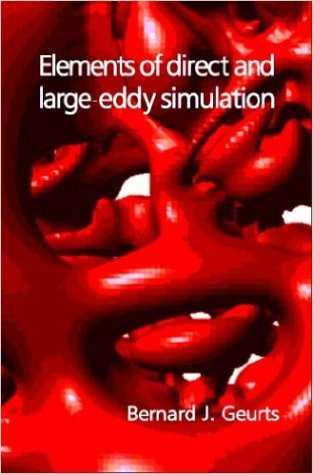
\includegraphics[height=0.5\textheight]{lesbook1.jpg}}
    \end{column}
  \end{columns}
\end{frame}

%------------------------------------------------

\begin{frame}{Recommended Textbooks}

\setlength{\fboxsep}{0pt}
\setlength{\fboxrule}{1pt}
\begin{columns}[T]
    \begin{column}{.75\textwidth}
      \begin{minipage}[c][.5\textheight][c]{\linewidth}
      \emph{\textbf{Large Eddy Simulation for Incompressible \\Flows}}\newline P. Sagaut (Springer, 2000), 556 pp.
      \end{minipage}
    \end{column}
    \begin{column}{.25\textwidth}
    \fbox{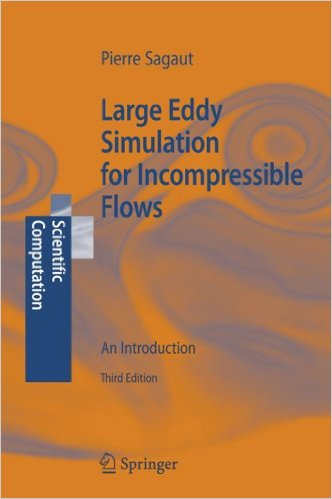
\includegraphics[height=0.5\textheight]{lesbook2.jpg}}
    \end{column}
  \end{columns}
\end{frame}

%------------------------------------------------

\begin{frame}{Recommended textbooks}

\setlength{\fboxsep}{0pt}
\setlength{\fboxrule}{1pt}
\begin{columns}[T]
    \begin{column}{.75\textwidth}
      \begin{minipage}[c][.47\textheight][c]{\linewidth}
      \emph{\textbf{Turbulent Flows}}\newline S. B. Pope (Cambridge University Press, 2000),\\ 771 pp.
      \end{minipage}
    \end{column}
    \begin{column}{.25\textwidth}
    \fbox{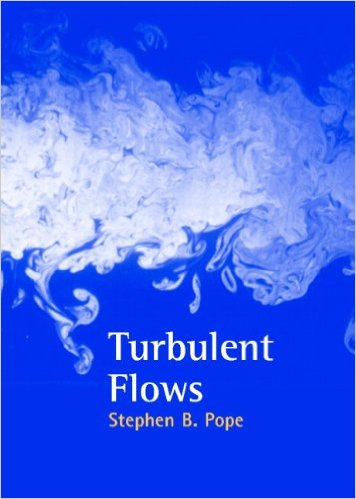
\includegraphics[height=0.47\textheight]{lesbook3.jpg}}
    \end{column}
  \end{columns}
\end{frame}

%------------------------------------------------

\begin{frame}{Useful courses}
\begin{itemize}
\item ME EN 5700/6700 - Fluid Dynamics
\item ME EN 7710 - Environmental Fluid Dynamics
\item ME EN 7720 - Turbulent Flows and Mixing
\end{itemize}
~\\~\\
Basically, you want to be familiar with the Navier-Stokes equations of motion and the general idea of turbulence.
\end{frame}

%------------------------------------------------

\begin{frame}{Grading}
\begin{itemize}
\item Homework - 40\%
\item Project \#1 - 25\%
\item Project \#2 - 35\%
\end{itemize}
~\\~\\
No exams!
\end{frame}

%------------------------------------------------
\subsection{Course Overview}
\begin{frame}{Course Description}
\begin{itemize}
\item This course covers topics related to Large-Eddy Simulation (LES), an advanced Computational Fluid Dynamics (CFD) technique. 
\item LES is quickly replacing traditional Reynolds Averaged Navier-Stokes (RANS) modeling as the method of choice for researchers and practitioners studying turbulent fluid flow phenomena in engineering and environmental problems.
\end{itemize}

\end{frame}

%------------------------------------------------

\begin{frame}{Course Description}
\begin{itemize}
\item LES explicitly solves for the larger scale turbulent motions that are highly dependent on boundary conditions, while using a turbulence model only for the smaller (and presumably more universal) motions. 
\item This is a distinct advantage over traditional RANS models where the effects of turbulence on the flow field are entirely dependent on the turbulence parameterizations.
\end{itemize}
\end{frame}

%------------------------------------------------

\begin{frame}{Course Objectives}
\begin{itemize}
\item Become familiar with the filtering concept in a turbulent flow and how the idea of scale separation forms the basis for LES.
\item Gain familiarity with the filtered forms of the conservation equations (e.g., mass, momentum, turbulent kinetic energy), how they are derived, and how the different terms in the equations can be interpreted.
\item Obtain a basic working knowledge of common subgrid-scale (SGS) parameterizations used in LES of turbulent flows.
\end{itemize}
\end{frame}

%------------------------------------------------

\begin{frame}{Course Objectives}
\begin{itemize}
\item Understand how to carry out \textit{a priori} analysis of SGS models from experimental and Direct Numerical Simulation (DNS) data sets.
\item Understand common techniques for \textit{a posteriori} evaluation of SGS models and what conditions are necessary and sufficient for a ``good'' SGS model.
\item Become familiar with LES SGS models and techniques used in specific flow cases of interest (e.g., isotropic turbulence, high-Reynolds number boundary layers,  turbulent reacting flows, etc.)
\end{itemize}
\end{frame}

%------------------------------------------------

\begin{frame}{Course Outline}
\begin{itemize}
\item Intro and motivation
\item Analysis tools
\item Turbulence and scale separation
\item Equations of motion
\item Filtering
\item Filtered equations of motion
\item Approaches to turbulence modeling
\item Numerics and LES
\item Basic SGS models
\begin{itemize}
\item eddy viscosity
\item similarity
\item nonlinear
\item mixed
\item dynamic models
\end{itemize}
\end{itemize}
\end{frame}

%------------------------------------------------

\begin{frame}{Course Outline}
\begin{itemize}
\item Using Fourier methods to simulate isotropic turbulence (Project \#1)
\item Evaluating LES (\textit{a posteriori})
\item Evaluating SGS models (\textit{a priori}, Project \#2)
\item Special Topics in LES (cover some set of the following examples)
\begin{itemize}
\item Boundary and initial conditions
\item Anisotropic models
\item Probability based methods
\item Lagrangian particle models
\item LES of compressible and/or reacting flows
\item LES case studies of interest
\end{itemize}
\end{itemize}
\end{frame}

%------------------------------------------------

\subsection{Coursework}
\begin{frame}{Homework}

What to expect:
\begin{itemize}
\item Approximately 3 homework assignments will be given during the semester. 
\item These assignments will focus on basic topics and ideas that will be needed in the projects (statistics of turbulence, filtering, power spectra estimation, model formulations, etc.). 
\item The assignments will be given throughout the semester when material is covered with an emphasis on the time period \textit{before} the 1st project.
\end{itemize}
\end{frame}

%------------------------------------------------

\begin{frame}{Homework}

Homework \#1
\begin{itemize}
\item Topics: \tabto*{50pt} Statistics, turbulence, spectra
\item Assigned:\tabto*{50pt} Thursday, August 23
\item Due:\tabto*{50pt} Thursday, September 15
\end{itemize}

Homework \#2
\begin{itemize}
\item Topics: \tabto*{50pt} 3D spectra from DNS data
\item Assigned:\tabto*{50pt} Thursday, September 15
\item Due:\tabto*{50pt} Thursday, October 6
\end{itemize}

Homework \#3
\begin{itemize}
\item Topics: \tabto*{50pt} SGS modeling
\item Assigned:\tabto*{50pt} Thursday, October 6
\item Due:\tabto*{50pt} Thursday, October 27
\end{itemize}
\end{frame}

%------------------------------------------------

\begin{frame}{Project \#1}

\begin{itemize}
\item Topic:\tabto*{50pt} \textit{a posteriori} study
\item Assigned:\tabto*{50pt} Tuesday, October 25
\item Due:\tabto*{50pt} Tuesday, November 22
\end{itemize}
\end{frame}

%------------------------------------------------

\begin{frame}{Project \#1}

The application of LES SGS models in 3D turbulence simulations. Students will be provided a basic 3D numerical code which they will add their own SGS models to and will then examine the effect of base model type, model coefficient specification, and grid resolution on the resolved simulated velocity fields. The project will be submitted in the form of a short report ($\sim4$ pages) outlining the basics of the simulation code used, the chosen SGS models, and the results of parameter studies.

\end{frame}

%------------------------------------------------

\begin{frame}{Project \#2}

\begin{itemize}
\item Topic:\tabto*{50pt} \textit{a priori} study
\item Assigned:\tabto*{50pt} Tuesday, November 1 or 8
\item Due:\tabto*{50pt} Thursday, December 8
\end{itemize}

\end{frame}

%------------------------------------------------

\begin{frame}{Project \#2}

Doing \textit{a priori} analysis of LES SGS models from experimental or numerical data.  Data sets from various experimental setups (high speed turbulence sensors, PIV) or high resolution DNS will be provided for students to use in the projects based on their research interests.  Alternatively, if students have appropriate data sets (experimental or numerical) that they wish to use for their project they will be free to do so. The project will be submitted in the form of a short report  ($\sim4$-$6$ pages) including: basics and background of the SGS models to be tested, a short description of the data set used in the analysis, and a short summary of key results/insights gained from the tests.  In addition to the project report, all students will be required to give a short presentation ($\sim15$ minutes) during the last weeks of class. 
\end{frame}

%------------------------------------------------
\section{LES Books}
\begin{frame}{LES Books}

\emph{\textbf{Elements of Direct and Large-Eddy Simulation}}\newline B.J. Geurts (R.T. Edwards, 2004), 329 pp.
~\\~\\
A readable book covering everything from turbulence theory to LES subgrid scale models and numerical techniques. It contains mostly incompressible flow with some applications to compressible flow. While not as complete as some other books (measured by the number of different methods), this is a nice first book to go over.	
\end{frame}

%------------------------------------------------
\begin{frame}{LES Books}

\emph{\textbf{Large Eddy Simulation for Incompressible Flows}}\newline P. Sagaut (Springer, 2000), 556 pp.
~\\~\\
Not really an introduction but more of a nice reference for LES SGS model techniques. It contains some turbulence theory but its best information is on filtering and SGS models. Probably the most complete collection of SGS models in any one place. It can be a difficult read due to the effort to include so many references.	
\end{frame}

%------------------------------------------------
\begin{frame}{LES Books}

\emph{\textbf{Turbulent Flows}}\newline S. B. Pope (Cambridge University Press, 2000), 771 pp.
~\\~\\
This book is not strictly speaking a book on LES. It is a book about incompressible turbulent flows that contains a very nice section on modeling. The modeling section includes a chapter on LES. The inclusion of general turbulence theory and LES together makes this book an ideal companion for texts that focus on LES and many times give brief or incomplete descriptions of the turbulent flow phenomena and mathematics the models are based on. Two related examples are isotropic turbulence theory (e.g., Kolmolgorov's hypothesis) and spectral analysis, both of which Pope gives excellent descriptions of.
\end{frame}

%------------------------------------------------
\begin{frame}{LES Books}

\emph{\textbf{Mathematics of Large Eddy Simulation of Turbulent Flows}}\newline Berselli, Iliescu, and Layton (Springer, 2005), 348 pp.
~\\~\\
This book is a nice text on LES focused on the mathematics of LES. It is written in the style of a math text book (complete with theorems, Lemmas, proofs and remark statements throughout the text). The mathematical viewpoint makes several sections very strong (including those related to filtering and approximate deconvolution) but at the same time makes the text a somewhat incomplete viewpoint of LES. For example phenomenological modeling strategies are not discussed. Some very important developments (e.g., dynamic modeling) are also missing from the textbook.
\end{frame}

%------------------------------------------------
\begin{frame}{LES Books}

\emph{\textbf{Large-Eddy Simulations of Turbulence}}\newline Lesieur, Metais, and Comte (Cambridge University Press, 2005), 219 pp.
~\\~\\
This is a shorter compact text on LES. Of the textbooks listed here, it contains one of the better descriptions of LES of compressible flow. It is also one of the better references for EDQNM (eddy-damped quasi-normal Markovian) theory, spectral LES, and structure function based SGS models. It is also the only text listed that explicitly discusses LES and atmospheric flows (although not in great detail).
\end{frame}

%------------------------------------------------
\begin{frame}{LES Books}

\emph{\textbf{Implicit Large Eddy Simulation}}\newline Grinstein,  Margolin, and Rider (Cambridge University Press, 2007), 546 pp.
~\\~\\
This book is a collection of papers on implicit LES techniques. The papers are logically chosen to give the reader a good overview of the development and motivation of this technique. This book is a nice starting point for a researcher interested in using ideas from those working in implicit LES. The first 2 chapters give a nice introduction to the technique and the motivations and historical developments.
\end{frame}

%------------------------------------------------
\begin{frame}{LES Books}

\emph{\textbf{Large Eddy Simulation of Complex Engineering and Geophysical Flows}}\newline Galperin and Orszag (Cambridge University Press, 2010), 624 pp.
~\\~\\
One of the first comprehensive books on LES, this book is a collection of chapters from different authors chosen and arranged in a logical way to include a wide range of topics starting at a basic level with an introduction to SGS modeling and a historical overview of the development of LES and then moving into specific topic areas in geophysics and engineering. It includes several nice papers on building-block (``canonical'' type) flows.
\end{frame}


%------------------------------------------------
\begin{frame}{LES Books}

\emph{\textbf{Large Eddy Simulation of Turbulent Incompressible Flows}}\newline Volker (Springer, 2004), 261 pp.
~\\~\\
A mathematically minded text this book contains a lot of information. It takes a similar approach to Berselli et al. (2006) but is harder to read. Its organization has more of a class notes feel than a well developed text. One unique feature is that it does contain a chapter devoted to testing many of the models discussed in the text in actual flows (2D and 3D mixing layers).
\end{frame}

%------------------------------------------------
\section{Intro to Turbulence} %
%------------------------------------------------

\begin{frame}{Leonardo da Vinci and Turbulence}

\setlength{\fboxsep}{0pt}
\setlength{\fboxrule}{1pt}
\begin{columns}[T]
    \begin{column}{.6\textwidth}
      \begin{minipage}[c][.6\textheight][c]{\linewidth}
      \begin{itemize}
      \item Lived from 1452--1519. 
      \item First to attempt scientific study of turbulence (\textit{turbolenza}). 
      \item He pioneered the notion of flow visualization to study turbulence. 
      \end{itemize}
      \end{minipage}
    \end{column}
    \begin{column}{.4\textwidth}
    \fbox{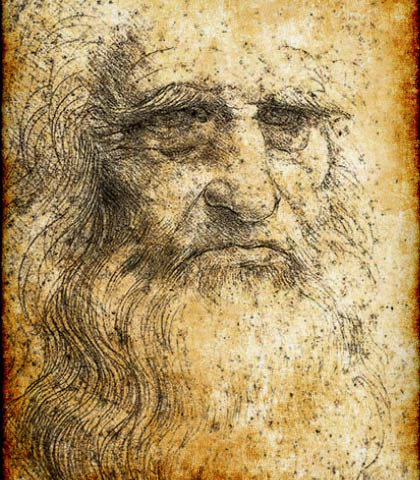
\includegraphics[width=\textwidth]{davinci1.jpg}}
    \end{column}
  \end{columns}

\end{frame}

%------------------------------------------------

\begin{frame}{Leonardo da Vinci and Turbulence}
  \setlength{\fboxsep}{0pt}
  \setlength{\fboxrule}{1pt}
  \begin{figure}[H]
  \centering
  \fbox{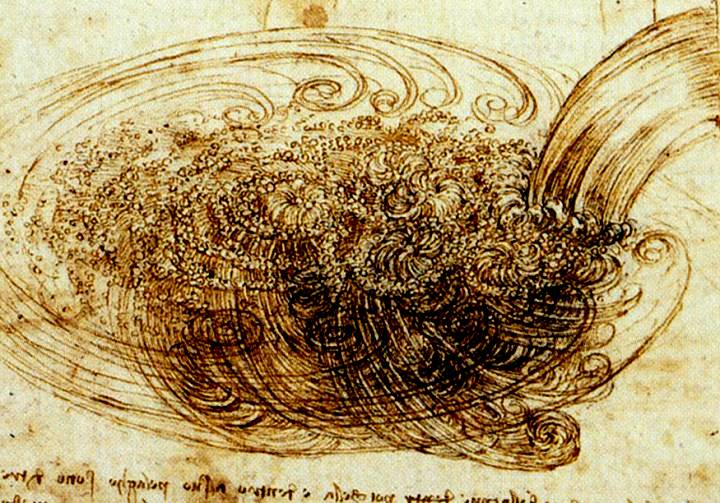
\includegraphics[width=0.4\textwidth]{davinci2.jpg}}
  \end{figure}
  
  He let water flow through a square hole into a pool and observed:
      \begin{fancyquotes}
      Observe the motion of the surface of the water, which resembles that of hair, which has two motions, of which one is caused by the weight of the hair, the other by the direction of the curls; thus the water has eddying motions, one part of which is due to the principal current, the other to random and reverse motion.	
      \end{fancyquotes}

Sounds very similar to Reynolds decomposition!

\end{frame}

%------------------------------------------------
\subsection{History}
\begin{frame}{Leonardo da Vinci and Turbulence}
  \setlength{\fboxsep}{0pt}
  \setlength{\fboxrule}{1pt}
  \begin{figure}[H]
  \centering
  \fbox{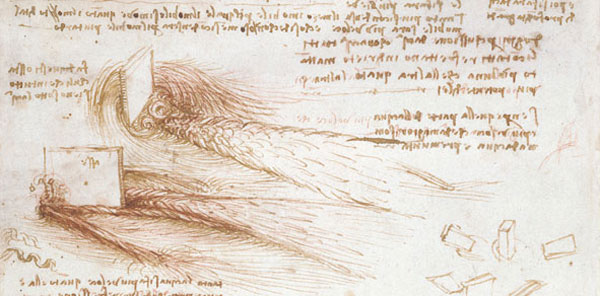
\includegraphics[width=0.5\textwidth]{davinci3.jpg}}
  \end{figure}
  
  In another, he placed obstacles in water:
      \begin{fancyquotes}
      So moving water strives to maintain the course pursuant to the power which occasions it, and if it finds an obstacle in its path it completes the span of the course it has commenced by a circular and revolving movement.	
      \end{fancyquotes}
Earliest reference to the importance of vortices!
\end{frame}

%------------------------------------------------

\begin{frame}{Leonardo da Vinci and Turbulence}
  \setlength{\fboxsep}{0pt}
  \setlength{\fboxrule}{1pt}
  \begin{figure}[H]
  \centering
  \fbox{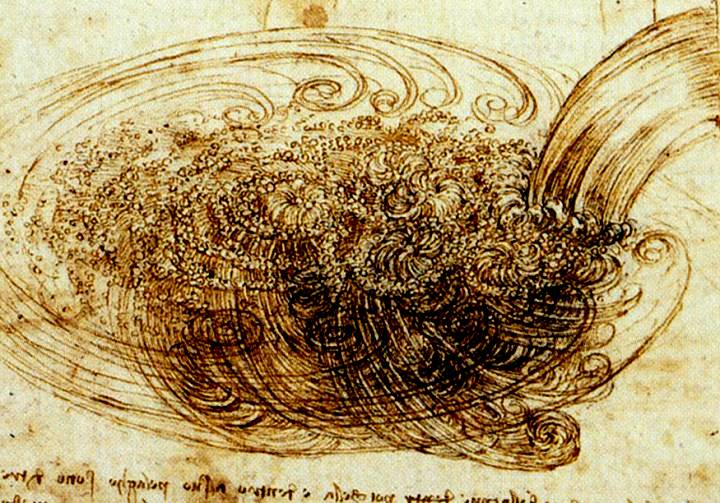
\includegraphics[width=0.5\textwidth]{davinci2.jpg}}
  \end{figure}
  
  In another, he placed obstacles in water:
      \begin{fancyquotes}
      ... the smallest eddies are almost numberless, and large things are rotated only by large eddies and not by small ones, and small things are turned by small eddies and large.	
      \end{fancyquotes}
Seems to hint at Richardson's turbulent cascade!
\end{frame}

%------------------------------------------------
\subsection{Motivation}
\begin{frame}{Why Turbulence?}

Why study turbulence?

\begin{itemize}
\item Turbulence is everywhere.
\item Smoke from a chimney, water flowing in a river, wind across a rough surface, flow around vehicles, combustion, solar wind.
\item Most real flows in environmental and engineering applications are turbulent. 
\item It remains one of the great unsolved problems in physics.
\end{itemize}

\end{frame}

%------------------------------------------------

\begin{frame}{Turbulence is Hard}

Werner Heisenberg, maybe:
\begin{fancyquotes}
	When I meet God, I am going to ask him two questions: Why relativity? And why turbulence? I really believe he will have an answer for the first.
\end{fancyquotes}

Horace Lamb, maybe:
\begin{fancyquotes}
	I am an old man now, and when I die and go to heaven there are two matters on which I hope for enlightenment. One is quantum electrodynamics, and the other is the turbulent motion of fluids. And about the former I am rather optimistic.
\end{fancyquotes}

\end{frame}

%------------------------------------------------

\subsection{Basic Properties}
\begin{frame}{Basic Observations of Turbulence}
\begin{itemize}
\item \textbf{Turbulence is random} \newline The properties of the fluid ($\rho$, $P$, $u$) at any given point ($x$,$t$) cannot be predicted. But statistical properties – time and space averages, correlation functions, and probability density functions – show regular behavior. The fluid motion is stochastic.
\item \textbf{Turbulence decays without energy input} \newline Turbulence must be driven or else it decays, returning the fluid to a laminar state.
\end{itemize}
\end{frame}

%------------------------------------------------

\begin{frame}{Basic Observations of Turbulence}
\begin{itemize}
\item \textbf{Turbulence displays scale-free behavior} \newline On all length scales larger than the viscous dissipation scale but smaller than the scale on which the turbulence is being driven, the appearance of a fully developed turbulent flow is the same.
\item \textbf{Turbulence displays intermittency} \newline ``Outlier'' fluctuations occur more often than chance would predict.
\end{itemize}
\end{frame}

%------------------------------------------------

\begin{frame}{Basic Observations of Turbulence}
  \begin{figure}[H]
  \centering
  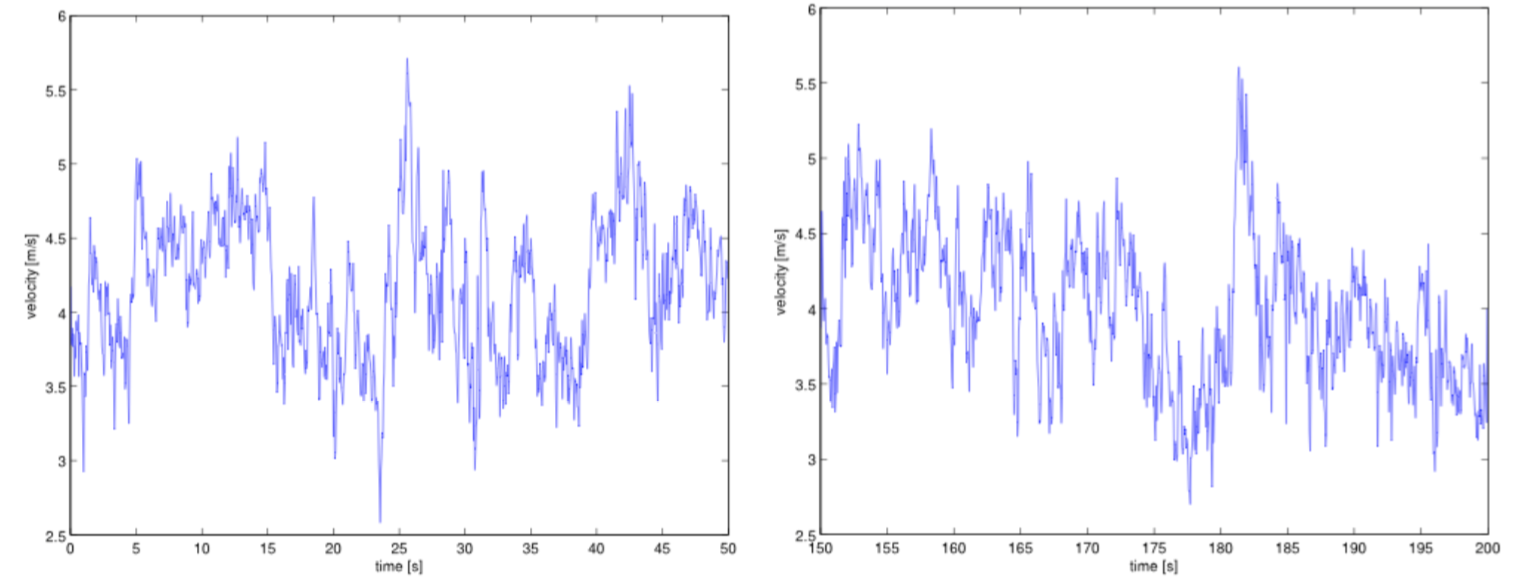
\includegraphics[width=1\textwidth]{timetrace1.png}
  \caption{\scriptsize Sonic anemometer data at 20Hz taken in the ABL.}
  \end{figure}
  
  The above figure is an example of the random nature of turbulent flows. Pope (2000) notes that using the term ``random'' means nothing more than that an event may or may not occur (it says nothing about the nature of the event)
  
\end{frame}

%------------------------------------------------

\begin{frame}{Basic Observations of Turbulence}
  \begin{figure}[H]
  \centering
  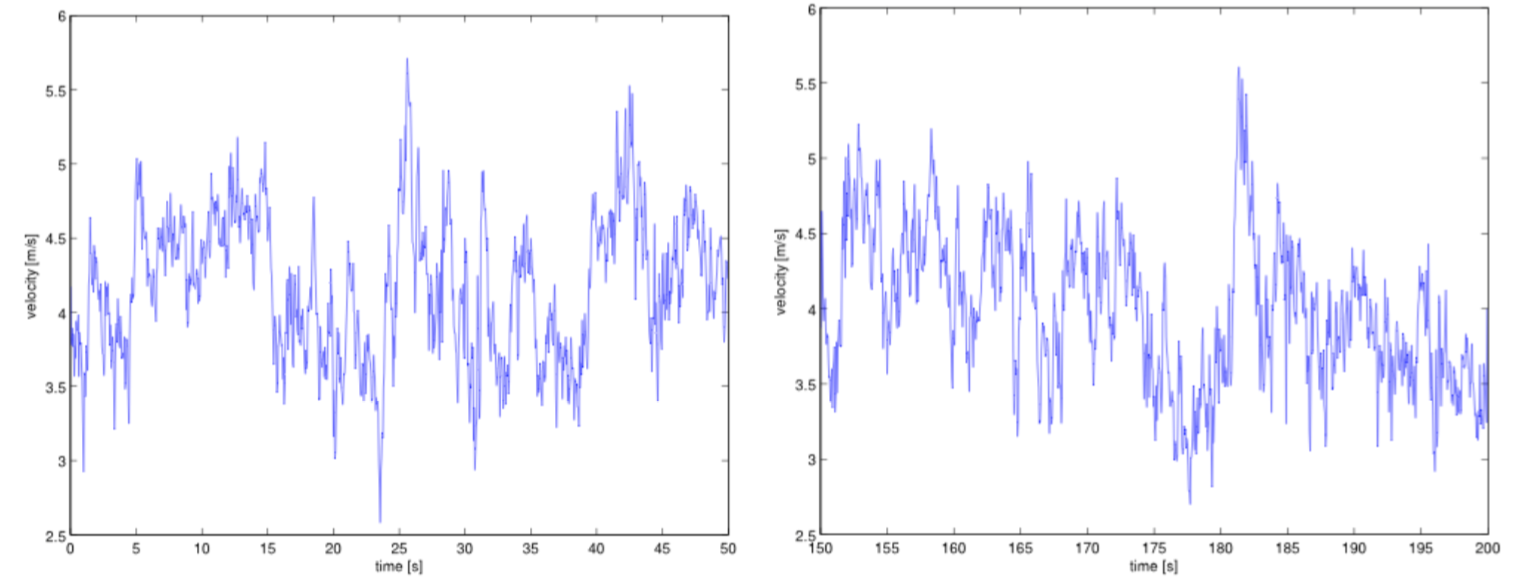
\includegraphics[width=1\textwidth]{timetrace1.png}
  \end{figure}
  We can observe a few things from the velocity time trace:
  \begin{itemize}
  \item The signal is highly disorganized and has structure on a wide range of scales (that is also disorganized).
  \item The signal appears unpredictable.
  \item Some of the properties of the signal appear to be reproducible.
  \end{itemize}
\end{frame}

%------------------------------------------------

\begin{frame}{What Makes Turbulence Such a Difficult Problem?}
  Beyond these properties, consider turbulent flow in general.
  \begin{itemize}
  \item To understand turbulence, we must resolve the entire range of temporal and spatial scales of the flow. 
  \item This range may be described by the Reynolds number (Re=$UL/\nu$) -- the ratio of inertia to viscous forces.  
  \item As Re increases, the range of length scales that must be increases dramatically.
  \end{itemize}
\end{frame}

%------------------------------------------------

\begin{frame}{What Makes Turbulence Such a Difficult Problem?}
  
  These scales often fall outside of those conditions that are easily measured:
  \begin{itemize}
  	\item high-velocities (aerodynamics)
  	\item high-temperatures (combustion)
  	\item hazardous substances (nuclear engineering)
  	\item very large scales (geophysics or astrophysics)
  \end{itemize}
  ~\\~\\
  This is why numerical simulations of turbulent flows are important!
  
  
\end{frame}


%------------------------------------------------

\end{document}

